\chapter{Ejemplo de uso con Netbeans} \label{}



	\section{Requisitos}

	\begin{enumerate}

	\item Necesitamos tener instalado kit de desarrollo Jdk de java que se puede descargar desde la página (http://www.oracle.com/technetwork/java/javase/downloads/).

	\item Necesitamos tener instalado el ambiente de desarrollo Netbeans que se puede descargar de la página (https://netbeans.org/downloads/).
	\end{enumerate}

	\section{Manualmente}\label{sec:manualInstall}
		Descargar el archivo .jar y agregarlo al folder /lib de la aplicación
		\begin{enumerate}
			\item Desde la página oficial de EQ PRO(ingenieria-eqpro.rhcloud.com) se puede descargar el archivo jar.

			\item Crear un nuevo proyecto desde Netbeans.

			\begin{center}
			  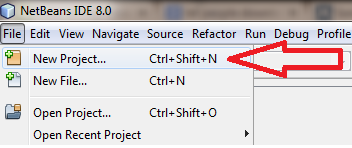
\includegraphics[scale=0.7]{new-proyect.png}
			\end{center}

			\item Elegir el tipo de aplicación java.application 
			\begin{center}
			  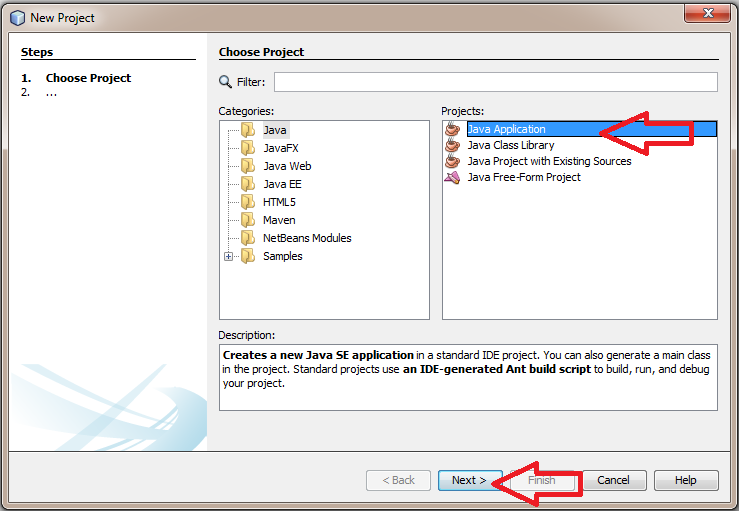
\includegraphics[scale=0.7]{application-type.png} 
			\end{center}
			\item Asignar el nombre del proyecto 
			\begin{center}
			  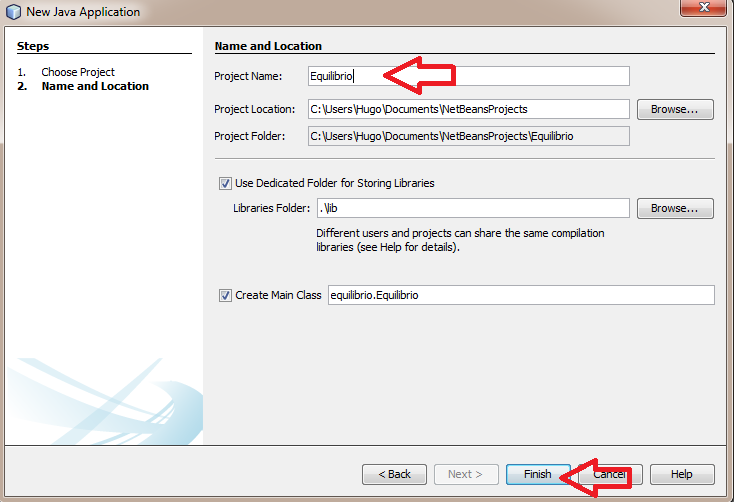
\includegraphics[scale=0.7]{proyect-name.png} 
			\end{center}
			\item En la pestaña proyectos de netbeans, con click derecho en la carpeta “Libraries” elegir la opción “Agregar jar/Folder “.
			\begin{center}
			  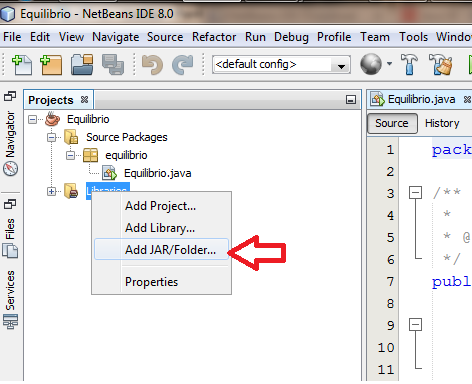
\includegraphics[scale=0.7]{add-jar.png} 
			\end{center}


			 \item Navegar entonces hasta la ruta donde se descargo el archivo jar. 

			\begin{center}
			  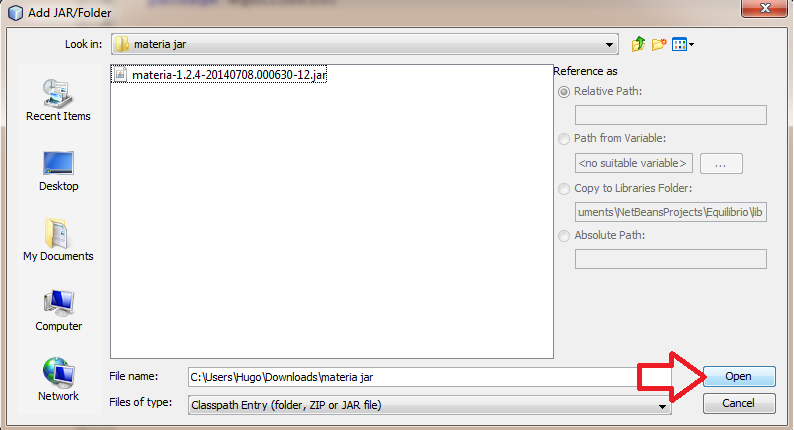
\includegraphics[scale=0.7]{select-materia-jar.png} 
			\end{center}

			Se puede ver entonces la librería agregada al proyecto.

			\begin{center}
			  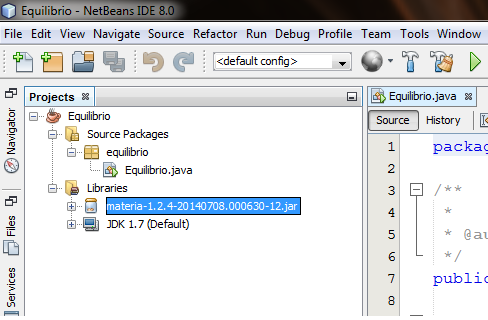
\includegraphics[scale=0.7]{library-added.png} 
			\end{center}
		\end{enumerate}

	\section{Maven}

		Desde maven utilizando el archivo pom.xml.
		    Crear nuevo proyecto :new proyect
		     Elegir la categoría ->Maven ->Java Applicationmaven java app
		    Elegir nombre del proyecto y dar click en finalizar.maven name
		    Podemos ver en la carpeta del proyecto la siguiente estructura
		\begin{verbatim}
		    Maven_Equilibrio
		    |-- pom.xml
		    `-- src
		        -- main
		           `-- java
		               `-- hugo
		                   `-- ejemplos
		                       `-- maven_equilibrio
		\end{verbatim}
		Abrimos el archivo pom.xml y agregamos las siguientes etiquetas


		\begin{lstlisting}[language=XML,morekeywords={repositories,
    repository,id,name,url,groupId,artifactId,dependencies,dependency}]
<dependencies>
  <dependency>
   <groupId>com.github.hugoredon</groupId>
   <artifactId>materia</artifactId>
   <version>1</version>
  </dependency>
</dependencies>
\end{lstlisting}


		5- Inmediatamente se ve agregada la dependencia Materia, cuando el proyecto se compile, se descargará el archivo jar automáticamente.

		maven materia added

		6.  Crear una clase java en cualquier paquete dentro de Source packages.maven create java class

		Escribimos dentro de esta clase el mismo código que en la entrada anterior.

	\section{Código}
		\begin{lstlisting}
			
		public class Equilibrio {
		 public static void main(String[] args) {
		 Compound agua = new Compound("agua");
		 agua.setCriticalTemperature(647.3);
		 agua.setCriticalPressure(2.212E7);
		 agua.setAcentricFactor(0.344861);
		 
		 Cubic cubicEquationOfState = EquationOfStateFactory.pengRobinsonBase();
		 Alpha alphaExpression = AlphaFactory.getStryjekAndVeraExpression();
		 
		 HeterogeneousSubstance substance =
		 new HeterogeneousSubstance(cubicEquationOfState, alphaExpression, agua);
		 double pressure = 101325;
		 substance.setPressure(pressure);
		 substance.bubbleTemperature();
		 double temperature = substance.getTemperature();
		 
		 System.out.println("(Presi|ó|n "+pressure+" [Pa])Temperatura de burbuja: " + temperature + "[K]");
		 }
		}

		\end{lstlisting}
		Ejecutamos el código y el resultado es:

		(Presión 101325.0 [Pa])Temperatura de burbuja: 374.5312063949659[K]